\section{Point Operations (V1)}
\begin{tabular}{ll}
  \parbox{8cm}{
    \subsection{Definition}
    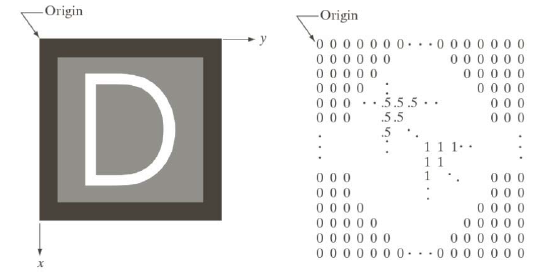
\includegraphics[width=7cm]{./images/image_definition.png}\\
    $M$ rows ($x$) and $N$ columns ($y$)
    } 
  & \parbox{11cm}{
    \subsection{Process}
    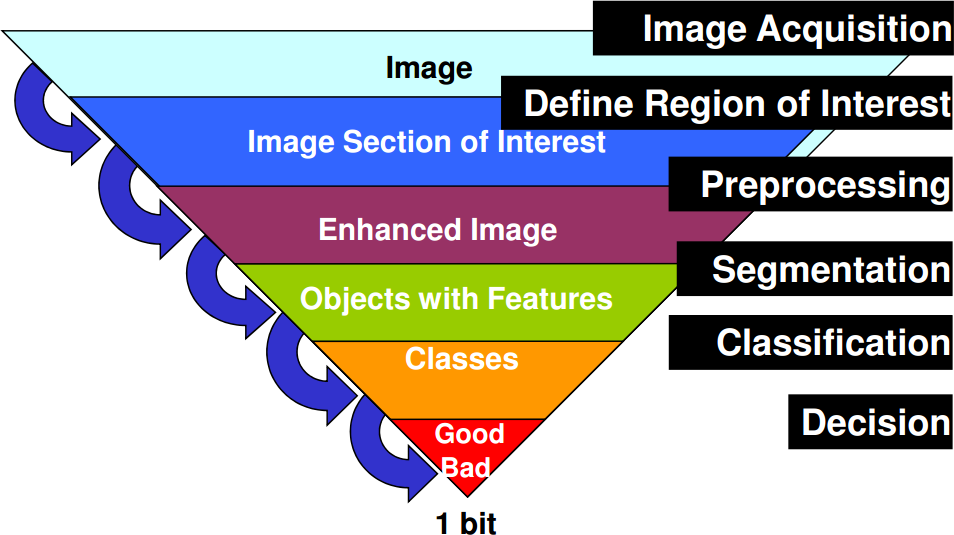
\includegraphics[width=10cm]{./images/image_process.png}
    }
  
\end{tabular}

Homogeneous operations don't depend on coordinates, but inhomogeneous do.



\skriptsubsection{Histogram}{120}

\begin{minipage}{11cm}

  $h(i) = $ number of pixels in $I$ with intensity value $i$\\
  
  Cumulative Histogram (Integral): $H(i) = \sum_{j=0}^i h(j)$ für $0 \leq i \leq K$
  
  Increasing Contrast: $f_c(a) = 1.5 a$\\
  Increasing Brightness: $f_b(a) = a + 10$\\
  Invert Image: $f_i(a) = a_{max} - a$\\

  \textbf{Optimize Dynamic Range} (saturate $s_{low}$\% and $s_{high}$ pixels): \\
  $\hat{a}_{low} = \min\{i | H(i) \geq M \cdot N \cdot s_{low}\}$\\
  $\hat{a}_{high} = \min\{i | H(i) \leq M \cdot N \cdot s_{high}\}$\\
  
  $f_{mac}(a) = \begin{cases}
  a_{min} & \text{ for } a \leq \hat{a}_{low}\\
  a_{min} + (a-a_{low}) \frac{a_{max} - a_{min}}{a_{high} - a_{low}} & \text{ for } \hat{a}_{low} < a < \hat{a}_{high}\\
  a_max & \text{ for } \hat{a}_{high}
  \end{cases}$
  
  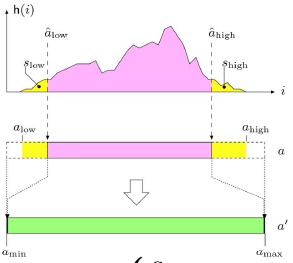
\includegraphics[width=8cm]{./images/automatic_contrast.png}
\end{minipage}
\begin{minipage}{7cm}
  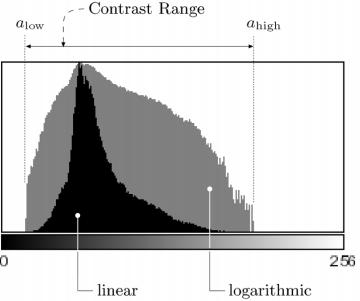
\includegraphics[width=8cm]{./images/contrast.png}

  \textbf{Histogram Equalisation:}\\
  $H(a) = H_{eq}(a')$\\
  $a' = H(a) \frac{255}{M \cdot N}$\\
  $H_{eq}(i) = M \cdot N \cdot i$\\
  $H(a) = a' \frac{M \cdot N}{255} $
  
  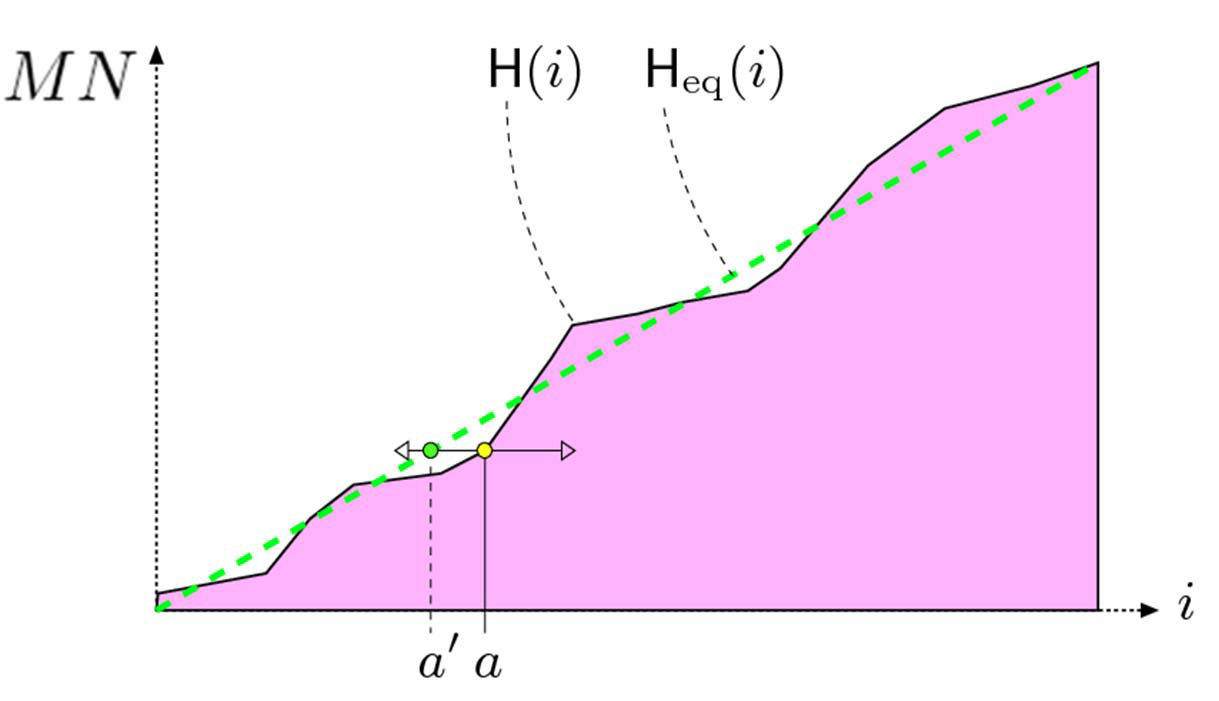
\includegraphics[width=7cm]{./images/histogram_equalisation.png}
\end{minipage}